
\documentclass[acmtog]{acmart}
% Title portion
\usepackage{indentfirst}
\setlength{\parindent}{2em}
\usepackage{listings}

\title{Assignment 1 : Geometric Modeling} 
\author{Name:\quad WenJi Liu  \\ student number:\quad 13611756
	\\email:\quad liuwj@shanghaitech.edu.cn}

% Document starts
\begin{document}
\maketitle

\vspace*{2 ex}


\section{Introduction}
 In this technical report, i  construct triangle meshes based on Bézier surfaces and then shade them with Ground lighting. \par Also, i implement the methods supporting camera controling (also rotation and translation) and texturing.
 \par Besides, i enabled the control points editing visually, and the surface will be automatically re-evaluated and re-meshed. 
 \par Finally, i implement a 2D Delaunay triangulation in triangle.h, but finally found it is not suitable for 3d cases and i post that on piazza.
 \par Thus i just do basic triangulation. When i consider delaunay property, as long as two triangles are not on the plane, they satisfy delaunay property. Since the bezier surface is curved, delaunay property always holds.
\section{Implementation Details}
\subsection{Bezier Surface generation}
To draw a bezier surface , we start with control points and evaluate bezier curves twice to get a bezier point.( first u then v).
\subsubsection{Eval Bezier Curve } x
\par First i complete the last interploration of bezier curve 
\begin{lstlisting}[frame=single,breaklines=true,language=c++,basicstyle=\footnotesize\ttfamily]
inline glm::vec3 mlBezier::derivBezier(const glm::vec3 * P, const float & t)
{
return (1 - t)*P[0] + t*P[1];
}
\end{lstlisting}
\par Then i do bezier interploration recursively,starting from controlpoints.
\begin{lstlisting}[frame=single,breaklines=true,language=c++,basicstyle=\footnotesize\ttfamily]
glm::vec3 mlBezier::mlEvalBezierCurve(const glm::vec3 * P, const float & t ,int input_length,bool getTagent)
{
if (input_length == 2) {
	if (getTagent==true) {
		return glm::normalize(P[0] - P[1]);

	}else {
		return derivBezier(P,t);
	}
}else {
	glm::vec3 * out_Points = new glm::vec3[input_length - 1];
	glm::vec3 P1, P2;
	for (int i = 0; i < input_length-1; i++) {
		P1 = P[i]; P2 = P[i + 1];
	out_Points[i] = (1 - t)*P1 + t*P2;
	}
	return mlEvalBezierCurve(out_Points, t,input_length-1,getTagent);
}
}
\end{lstlisting}
\par getTagent is a flag to return the tagent vector on that point instead of returning that point.\par input\_length is the number of points in P.\par At each iteration, the point numbers will decrease by one.With this function, we can get a point or its tagent vector.
\begin{lstlisting}[frame=single,breaklines=true,language=c++,basicstyle=\footnotesize\ttfamily]
glm::vec3 mlBezier::mlEvalBezierPatch(const glm::vec3 * controlPoints, const float & u, const float & v)
{
	glm::vec3 Pu[4];
	for (int i = 0; i < 4;i++) {
		glm::vec3 curveP[4];
		curveP[0] = controlPoints[i * 4];
		curveP[1] = controlPoints[i * 4+1];
		curveP[2] = controlPoints[i * 4+2];
		curveP[3] = controlPoints[i * 4+3];
		Pu[i] = mlEvalBezierCurve(curveP, u,4,false);
	}
	return mlEvalBezierCurve(Pu, v,4,false);
}
\end{lstlisting}
\par To get tagent vector. Calculate from tagent vecors on the controlPoints.And interplorate it from the nearst two tagent vector.
\begin{lstlisting}[frame=single,breaklines=true,language=c++,basicstyle=\footnotesize\ttfamily]
glm::vec3 mlBezier::dUBezier(const glm::vec3 * controlPoints, const float & u, const float & v)
{
	glm::vec3 Pu[4];
	for (int i = 0; i < 4; i++) {
		glm::vec3 curveP[4];
		curveP[0] = controlPoints[i * 4];
		curveP[1] = controlPoints[i * 4 + 1];
		curveP[2] = controlPoints[i * 4 + 2];
		curveP[3] = controlPoints[i * 4 + 3];
		Pu[i] = mlEvalBezierCurve(curveP, u, 4,true);
	}
	int pre = floor(v * 4);
	float t = v * 4 - pre;
	int next = ceil(v * 4);
	return Pu[pre] * (1 - t) + t*Pu[next];
}
\end{lstlisting}
\par Now that we can eval bezier points smoothly.To generate the mesh, we should specify (u,v) to generate a point with normal and st.
\par Normal is generating by cross product from two tagent vector.
\begin{lstlisting}[frame=single,breaklines=true,language=c++,basicstyle=\footnotesize\ttfamily]
void mlBezier::mlCreateBeizermesh()
{
	P.clear(); N.clear(); st.clear();
	float step = 1/sqrt(divs);
	for (float v = 0; v <= 1; v += step) {
		for (float u = 0; u <= 1; u += step) {
			glm::vec3 p = mlEvalBezierPatch(controlPoints, u, v);
			P.push_back(p);
			N.push_back(
			glm::normalize(
			glm::cross(dUBezier(controlPoints, u, v), dVBezier(controlPoints, u, v))
			)
			);
			st.push_back(glm::vec2(u, v));
			
		}
	}
}
\end{lstlisting}
\par to draw the surface out.
\begin{lstlisting}[frame=single,breaklines=true,language=c++,basicstyle=\footnotesize\ttfamily]
void mlBezier::mlTriangularization()
{
	indicesofControlpoints.clear();
	for (int j = 0; j < 3; j++)
	{
		for (int i = 0; i < 3; i++)
		{
			int ind = j * 4 + i;
			indicesofControlpoints.push_back(ind);
			indicesofControlpoints.push_back(ind + 1);
			indicesofControlpoints.push_back(ind + 5);
			indicesofControlpoints.push_back(ind + 4);
		}
	}
	indicesofP.clear();
	int div = sqrt(divs);
	indicesofP.clear();
	for (int j = 0; j < div; j++)
	{
		for (int i = 0; i < div; i++)
		{
			int ind = j * (div+1) + i;
			indicesofP.push_back(ind);
			indicesofP.push_back(ind + 1);
			indicesofP.push_back(ind + (div + 1));
			
			indicesofP.push_back(ind + 1);
			indicesofP.push_back(ind + (div + 2));
			indicesofP.push_back(ind + (div + 1));
		}
	}
}
\end{lstlisting}
\begin{lstlisting}[frame=single,breaklines=true,language=c++,basicstyle=\footnotesize\ttfamily]
void drawBezierSurface(mlBezier &mlbezier)
{
	glm::vec3 points_pos[3], points_norm[3];glm::vec2 points_tex[3];
	for (size_t i = 0; i < mlbezier.indicesofP.size(); i += 3) {
		points_pos[0] = mlbezier.P[mlbezier.indicesofP[i]];
		points_norm[0] = mlbezier.N[mlbezier.indicesofP[i]];
		points_tex[0] = mlbezier.st[mlbezier.indicesofP[i]];

		glColor3f(1, 1, 1);
		glBegin(GL_TRIANGLES);
		glNormal3f(points_norm[0].x, points_norm[0].y, points_norm[0].z);
		glTexCoord2f(points_tex[0].x, points_tex[0].y);
		glVertex3f(points_pos[0].x, points_pos[0].y, points_pos[0].z);
		glEnd();
		...
	}
}
\end{lstlisting}
This function setting up the points based on the division ,for example 6x6 or 9x9. it suits all.
\subsubsection{curve result}x
\par From the front view, the surface is smooth.\\
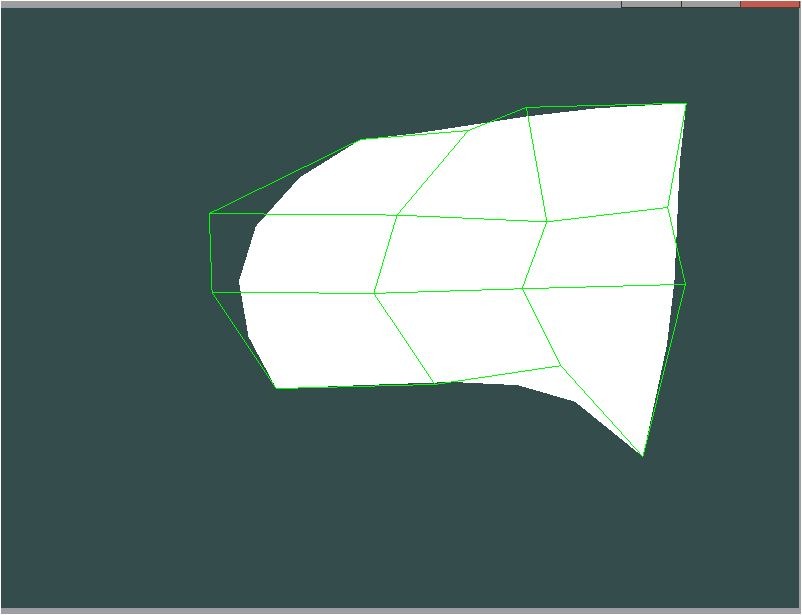
\includegraphics[scale=0.5]{0}
\par From the back view, the surface satisfy the division=25.\\
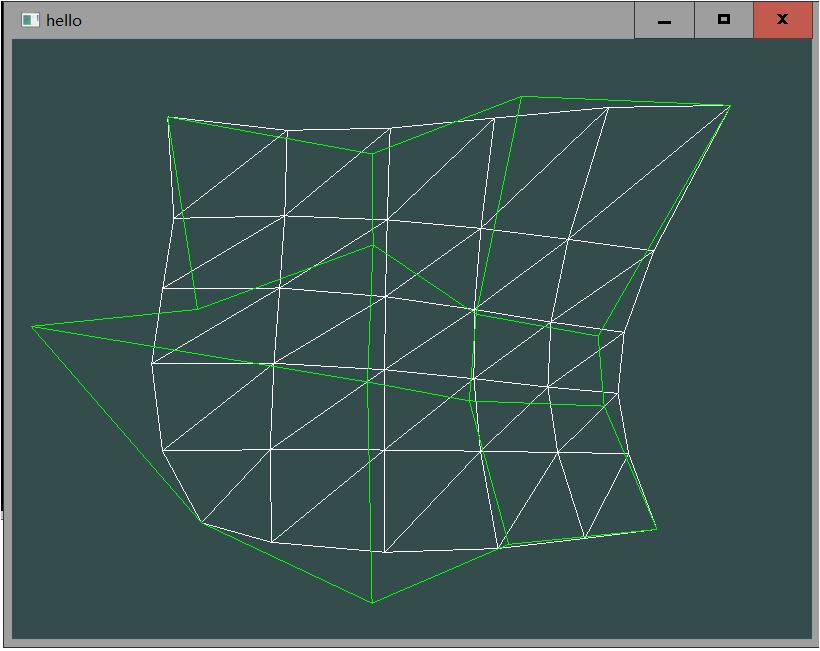
\includegraphics[scale=0.5]{1}
\subsection{Camera movement}
\par I defined several global variables.
\begin{lstlisting}[frame=single,breaklines=true,language=c++,basicstyle=\footnotesize\ttfamily]
//Setting up camera 
// for translating the camera
glm::vec3 cameraPos = glm::vec3(0.0f, 0.0f, 3.0f);
glm::vec3 cameraFront = glm::vec3(0.0f, 0.0f, -1.0f);
glm::vec3 cameraUp = glm::vec3(0.0f, 1.0f, 0.0f);

glm::mat4 model ,view, projection;
// fo smoothing 
float deltaTime = 0;
float lastFrame = 0;
// for rotating the camera
float pitch = 0;
float yaw = -90.0f;
// for mouse input 
float lastX = 400, lastY = 300;
bool firstMouse = true;
// for scene scaling 
float fov = 45.0f;
glm::vec3 lightPos(1.2f, 1.0f, 2.0f);
\end{lstlisting}
\par also two global functions
\begin{lstlisting}[frame=single,breaklines=true,language=c++,basicstyle=\footnotesize\ttfamily]
void initPMV()
{
	glMatrixMode(GL_PROJECTION);
	glLoadIdentity();

	gluPerspective(60, SCR_WINDTH / SCR_HEIGHT, 0.1, 100);

	glMatrixMode(GL_MODELVIEW);
	glLoadIdentity();
	gluLookAt
	(0, 0, 7.5,
	0, 0, 0,
	0, 1, 0
	);
}
void changePMV() {
	glMatrixMode(GL_PROJECTION);
	glLoadIdentity();
	gluPerspective(fov, SCR_WINDTH / SCR_HEIGHT, 0.1, 100);
	glMatrixMode(GL_MODELVIEW);
	glLoadIdentity();
	gluLookAt
	(cameraPos.x,cameraPos.y,cameraPos.z,
	cameraPos.x+cameraFront.x, cameraPos.y + cameraFront.y, cameraPos.z + cameraFront.z,
	cameraUp.x,cameraUp.y,cameraUp.z
	);
	view = glm::lookAt(cameraPos, cameraPos + cameraFront, cameraUp);
	projection = glm::perspective(glm::radians(fov), (float)(SCR_WINDTH / SCR_HEIGHT), 0.1f, 100.0f);
}
\end{lstlisting}
Fill in the void processInput(Window * window)
\begin{lstlisting}[frame=single,breaklines=true,language=c++,basicstyle=\footnotesize\ttfamily]


void processInput(GLFWwindow *window)
{

float cameraSpeed = 2.5f* deltaTime; // adjust accordingly
if (glfwGetKey(window, GLFW_KEY_ESCAPE) == GLFW_PRESS)
glfwSetWindowShouldClose(window, true);
if (glfwGetKey(window, GLFW_KEY_W) == GLFW_PRESS)
cameraPos += cameraSpeed * cameraFront;
if (glfwGetKey(window, GLFW_KEY_S) == GLFW_PRESS)
cameraPos -= cameraSpeed * cameraFront;
if (glfwGetKey(window, GLFW_KEY_A) == GLFW_PRESS)
cameraPos -= glm::normalize(glm::cross(cameraFront, cameraUp)) * cameraSpeed;
if (glfwGetKey(window, GLFW_KEY_D) == GLFW_PRESS)
cameraPos += glm::normalize(glm::cross(cameraFront, cameraUp)) * cameraSpeed;

}
\end{lstlisting}
\par Now press WASD to translate the camera, indeed it's changing the view matrix.
\par To support camera rotating. 
\begin{lstlisting}[frame=single,breaklines=true,language=c++,basicstyle=\footnotesize\ttfamily]
void mouse_callback(GLFWwindow* window, double xpos, double ypos)
{
if (firstMouse) // Initialization 
{
	lastX = xpos;
	lastY = ypos;
	firstMouse = false;
}
// calculate the mouse movement
float xoffset = xpos - lastX;
float yoffset = lastY - ypos; 
lastX = xpos;
lastY = ypos;

float sensitivity = 0.05f;
xoffset *= sensitivity;
yoffset *= sensitivity;

yaw += xoffset;
pitch += yoffset;
\\restrict the camera not to rotate to backwards
if (pitch > 89.0f)
pitch = 89.0f;
if (pitch < -89.0f)
pitch = -89.0f;

glm::vec3 front;
front.x = cos(glm::radians(pitch)) * cos(glm::radians(yaw));
front.y = sin(glm::radians(pitch));
front.z = cos(glm::radians(pitch)) * sin(glm::radians(yaw));
\\set the camera front
cameraFront = glm::normalize(front);
}
\end{lstlisting}
In this function, i calculate the relative mouse movement  and change the yaw/pitch of the camera. 
To further support scaling , use mouse scroll event to change the fov of camera.
\begin{lstlisting}[frame=single,breaklines=true,language=c++,basicstyle=\footnotesize\ttfamily]
glfwSetScrollCallback(window, scroll_callback);
void scroll_callback(GLFWwindow* window, double xoffset, double yoffset) {
	if (fov >= 1.0f && fov <= 45.0f)
		fov -= yoffset;
	if (fov <= 1.0f)
		fov = 1.0f;
	if (fov >= 45.0f)
		fov = 45.0f;
}
\end{lstlisting}
\subsection{Gourand Lighting with OpenGL}
First specify material of light source and obect.
\begin{lstlisting}[frame=single,breaklines=true,language=c++,basicstyle=\footnotesize\ttfamily]
GLfloat sun_light_position[] = { 0.0f, 0.0f, 12.0f, 0.0f };
GLfloat sun_light_ambient[] = { 0.0f, 0.0f, 0.0f, 1.0f };
GLfloat sun_light_diffuse[] = { 1.0f,  0.0f, 1.0f, 1.0f };
GLfloat sun_light_specular[] = { 1.0f, 1.0f, 0.0f, 1.0f };

GLfloat earth_mat_ambient[] = { 1.0f, 1.0f, 1.0f, 1.0f };
GLfloat earth_mat_diffuse[] = { 0.0f, 0.0f, 0.5f, 1.0f };
GLfloat earth_mat_specular[] = { 1.0f, 0.0f, 0.0f, 1.0f };
GLfloat earth_mat_emission[] = { 0.0f, 0.0f, 0.0f, 1.0f };
GLfloat earth_mat_shininess = 30.0f;
\end{lstlisting}
\par Add following codes into drawBezierSurface()
\begin{lstlisting}[frame=single,breaklines=true,language=c++,basicstyle=\footnotesize\ttfamily]
glMaterialfv(GL_FRONT, GL_AMBIENT, earth_mat_ambient);
glMaterialfv(GL_FRONT, GL_DIFFUSE, earth_mat_diffuse);
glMaterialfv(GL_FRONT, GL_SPECULAR, earth_mat_specular);
glMaterialfv(GL_FRONT, GL_EMISSION, earth_mat_emission);
glMaterialf(GL_FRONT, GL_SHININESS, earth_mat_shininess);
\end{lstlisting}
\par in AddLight(), turn on lighting.
\begin{lstlisting}[frame=single,breaklines=true,language=c++,basicstyle=\footnotesize\ttfamily]
void AddLight(mlBezier &mlbezier)
{
	glLightfv(GL_LIGHT0, GL_POSITION, sun_light_position);
	glLightfv(GL_LIGHT0, GL_AMBIENT, sun_light_ambient);
	glLightfv(GL_LIGHT0, GL_DIFFUSE, sun_light_diffuse);
	glLightfv(GL_LIGHT0, GL_SPECULAR, sun_light_specular);
	glEnable(GL_LIGHTING);
	glEnable(GL_LIGHT0);
}
\end{lstlisting}
\subsubsection{Lighting Result}x\\
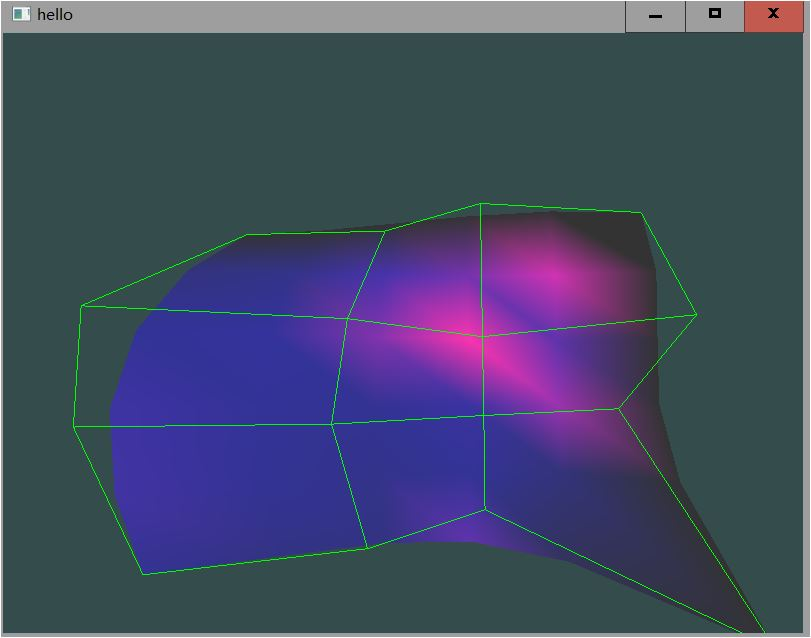
\includegraphics[scale=0.5]{2}
\par the purple part is specular part, the basis diffuse is blue.
\subsection{Texturing}
Initialize the texuture and set parameters.
\begin{lstlisting}[frame=single,breaklines=true,language=c++,basicstyle=\footnotesize\ttfamily]
void initTexture(unsigned int &texture)
{
	int width, height, nrChannels;
	unsigned char *data = stbi_load("resource/textures/container.jpg", &width, &height, &nrChannels, 0);
	//bind it to texture
	glEnable(GL_TEXTURE_2D);
	glGenTextures(1, &texture);
	glBindTexture(GL_TEXTURE_2D, texture);
	// set the active texture
	glTexImage2D(GL_TEXTURE_2D, 0, GL_RGB, width, height, 0, GL_RGB, GL_UNSIGNED_BYTE, data);
	// sample: specify texture parameters
	glTexParameteri(GL_TEXTURE_2D, GL_TEXTURE_WRAP_S, GL_REPEAT);
	glTexParameteri(GL_TEXTURE_2D, GL_TEXTURE_WRAP_T, GL_REPEAT);
	glTexParameteri(GL_TEXTURE_2D, GL_TEXTURE_MAG_FILTER, GL_LINEAR);
	glTexParameteri(GL_TEXTURE_2D, GL_TEXTURE_MIN_FILTER, GL_LINEAR);
	stbi_image_free(data);
}
\end{lstlisting}
Since st is already setted in drawBezierSurface()
\begin{lstlisting}[frame=single,breaklines=true,language=c++,basicstyle=\footnotesize\ttfamily]
glTexCoord2f(points_tex[0].x, points_tex[0].y);
\end{lstlisting}
Bind Texture before drawing, then all should work as expected.\\
Add following code into  drawBezierSurface()
\begin{lstlisting}[frame=single,breaklines=true,language=c++,basicstyle=\footnotesize\ttfamily]
glBindTexture(GL_TEXTURE_2D, texture);
\end{lstlisting}
\subsubsection{Texture result}x\\
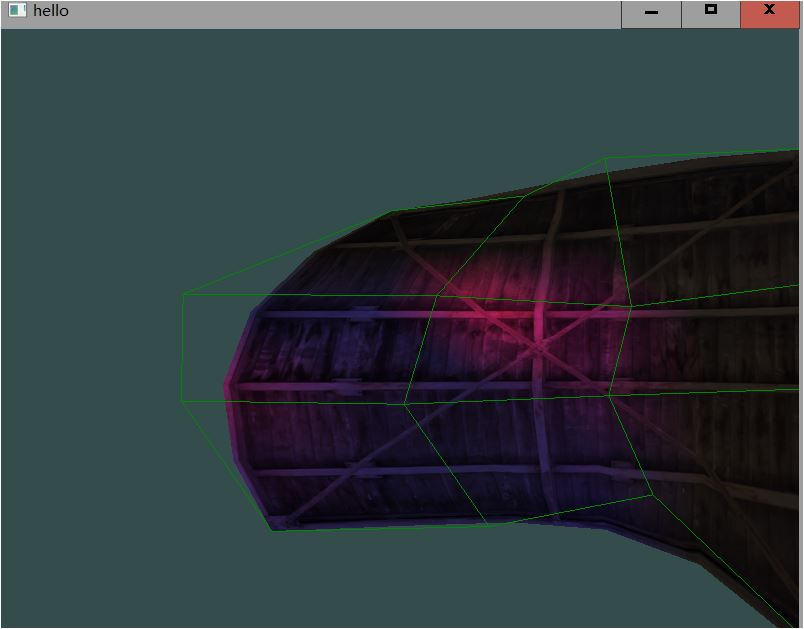
\includegraphics[scale=0.5]{3}
\subsection{Editing ControlPoints}
The main idea is to project all current 3d points back to screen space and select a point closest to the cursor position under certain threshold.
\par Then estiamte mouse movement until mouse release. Then get a estimated screen space point, and we projected it back to set the 3d controlPoints.
\par First, we register the mouse\_button\_callback() 
\begin{lstlisting}[frame=single,breaklines=true,language=c++,basicstyle=\footnotesize\ttfamily]
void mouse_button_callback(GLFWwindow* window, int button, int action, int mods);
glfwSetMouseButtonCallback(window, mouse_button_callback);
\end{lstlisting}
Use drag\_start and drag\_end to estimate the mouse movement during dragging. \\Use dragFlag to specify whether is on the process of dragging.
\begin{lstlisting}[frame=single,breaklines=true,language=c++,basicstyle=\footnotesize\ttfamily]
void mouse_button_callback(GLFWwindow* window, int button, int action, int mods)
{
	double xpos, ypos;
	glm::vec4 viewport = glm::vec4(0, 0, SCR_WINDTH, SCR_HEIGHT);
	glfwGetCursorPos(window, &xpos, &ypos);
	if (action == GLFW_PRESS) switch (button)
	{
		case GLFW_MOUSE_BUTTON_LEFT:
		if (dragFlag == false) {
			int ind = mlbezier.getSelectedControlPointIndice(xpos, ypos, view, projection, viewport);
			if (ind != -1) {
				dragFlag = true;
				drag_start = glm::vec2(xpos,viewport[3]- ypos);
				selected_index = ind;
			}
		}
		break;
		default:
		return;
	}
	
	if (action == GLFW_RELEASE) switch (button)
	{
		case GLFW_MOUSE_BUTTON_LEFT:
		if (dragFlag ==true&&selected_index!=-1) {
			drag_end = glm::vec2(xpos, viewport[3] - ypos);
			mlbezier.updateControlPointPosition(selected_index, (drag_end - drag_start),view,projection,viewport);
			mlbezier.mlCreateBeizermesh();//Recreate mesh and triangularization
			mlbezier.mlTriangularization();
			selected_index = -1;
			dragFlag = false;
		}
		break;
		default:
		return;
	}
	return;
}
\end{lstlisting}
Note that due to the windows screen coordinate is upside down of opengl screen coordiante,we should do `Height - ypos` to convert to opengl coordiante.
\\Then we can use glm::project and glm::unproject currently.
\begin{lstlisting}[frame=single,breaklines=true,language=c++,basicstyle=\footnotesize\ttfamily]
int mlBezier::getSelectedControlPointIndice(int posX, int posY,glm::mat4 view,glm::mat4 projection,glm::vec4 viewport)
{
	float minDistance = 65536;
	int ind = -1;
	float thres = 20;
	for (int i = 0; i < controlPointsNums; i++) {
		glm::vec3 pos = glm::project(controlPoints[i], view, projection, viewport);
		float distance =glm::distance(glm::vec2(posX, viewport[3] - posY), glm::vec2(pos.x,pos.y));
		if (distance < minDistance && distance<thres) {
			minDistance = distance;
			ind = i;
		}
	}
	return ind;
}
\end{lstlisting}
\begin{lstlisting}[frame=single,breaklines=true,language=c++,basicstyle=\footnotesize\ttfamily]
void mlBezier::updateControlPointPosition(int selectedInd,glm::vec2 moveDistance,glm::mat4 view, glm::mat4 projection, glm::vec4 viewport)
{
	glm::vec3 pos = glm::project(controlPoints[selectedInd], view, projection, viewport);
	glm::vec3 newprojected = glm::vec3(pos.x + moveDistance.x, pos.y + moveDistance.y, pos.z);
	this->controlPoints[selectedInd] = glm::unProject(newprojected,view, projection, viewport);
} 
\end{lstlisting}
Thus the controlpoints editing should work.
\subsubsection{Editing Result}x
Before editing.\\
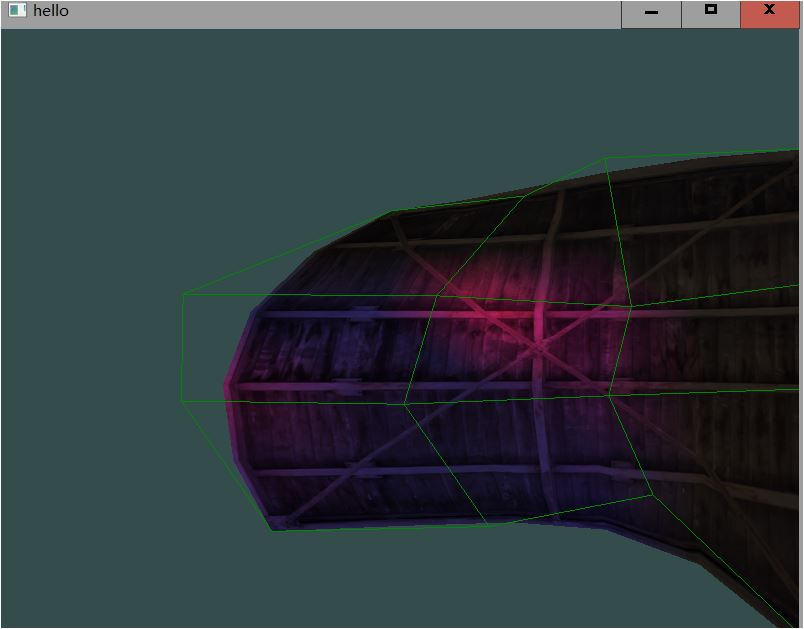
\includegraphics[scale=0.5]{3}\\
After editing.\\
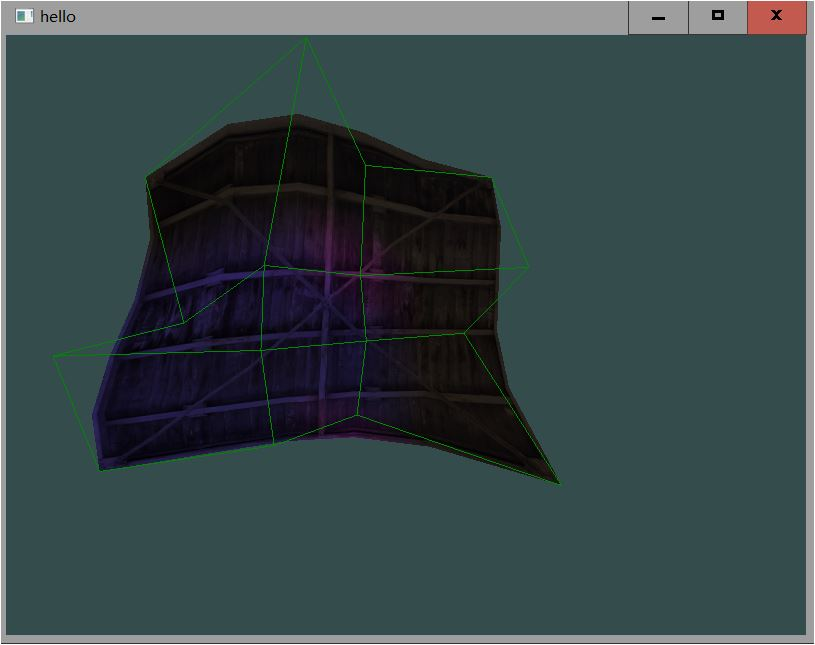
\includegraphics[scale=0.5]{4}
\end{document}
